% This LaTeX was auto-generated from MATLAB code.
% To make changes, update the MATLAB code and export to LaTeX again.

\documentclass{article}

\usepackage[utf8]{inputenc}
\usepackage[T1]{fontenc}
\usepackage{lmodern}
\usepackage{graphicx}
\usepackage{color}
\usepackage{hyperref}
\usepackage{amsmath}
\usepackage{amsfonts}
\usepackage{epstopdf}
\usepackage[table]{xcolor}
\usepackage{matlab}

\sloppy
\epstopdfsetup{outdir=./}
\graphicspath{ {./topt_p1_andres_herencia_antonio_fernandez_images/} }

\matlabhastoc

\begin{document}

\label{T_52757AB5}
\matlabtitle{\textbf{PRACTICE 1 - OPTIMIZATION TECHNIQUES}}

\begin{par}
\begin{flushleft}
\textbf{Andrés Herencia y Antonio Fernández}
\end{flushleft}
\end{par}

\begin{par}
\begin{flushleft}
\textbf{MUTECI 2023-2024}
\end{flushleft}
\end{par}

\matlabtableofcontents{Table of Contents}

\label{H_067E0EA8}
\matlabheading{Exercise 1}

\begin{par}
\begin{flushleft}
Given the following values:
\end{flushleft}
\end{par}

\begin{matlabcode}
x = [2 4 6 8]'
\end{matlabcode}
\begin{matlaboutput}
x = 4x1    
     2
     4
     6
     8

\end{matlaboutput}
\begin{matlabcode}
y = [3 2 5 6]'
\end{matlabcode}
\begin{matlaboutput}
y = 4x1    
     3
     2
     5
     6

\end{matlaboutput}

\begin{par}
\begin{flushleft}
Determine the regression line
\end{flushleft}
\end{par}

\begin{par}
$$y=\beta_0 \;+\;\beta_1 x$$
\end{par}

\begin{par}
\begin{flushleft}
Using MATLAB with a pre-built function and another function for the linear regression model.
\end{flushleft}
\end{par}

\label{H_B923E66F}
\matlabheadingtwo{Solution}

\label{H_F0977E52}
\matlabheadingthree{Original data}

\begin{par}
\hfill \break
\end{par}

\begin{matlabcode}
clf;
plot(x,y,'b+')
grid on
xlim([min(x)*0.8,max(x)*1.2])
ylim([min(y)*0.8,max(y)*1.2])
\end{matlabcode}
\begin{center}
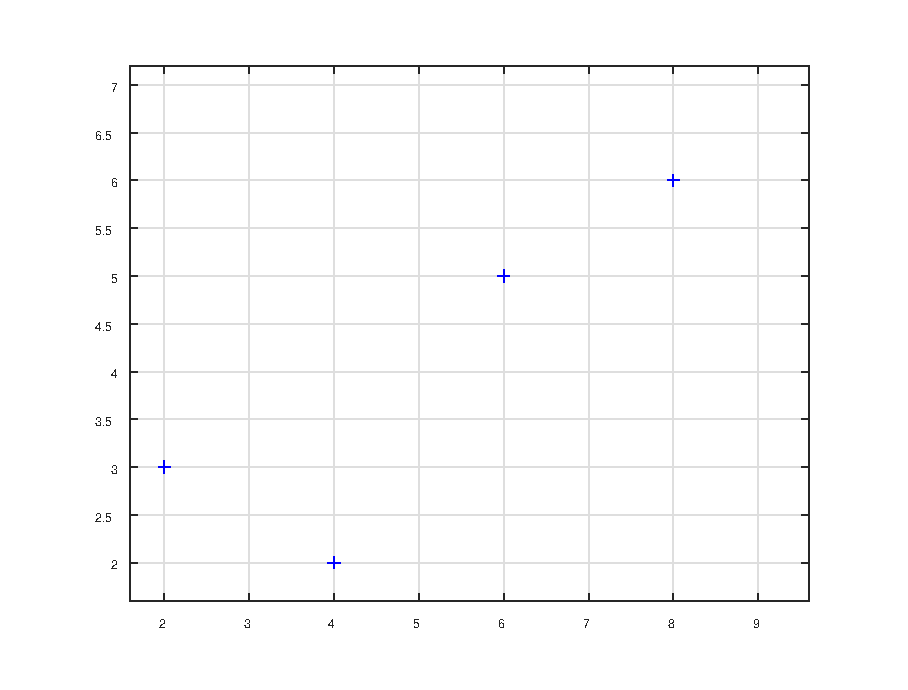
\includegraphics[width=\maxwidth{56.196688409433015em}]{figure_0.eps}
\end{center}

\label{H_AAFB13CE}
\matlabheadingthree{With \texttt{regress} function}

\begin{par}
\hfill \break
\end{par}

\begin{matlabcode}
X = [ones(length(x),1),x]
\end{matlabcode}
\begin{matlaboutput}
X = 4x2    
     1     2
     1     4
     1     6
     1     8

\end{matlaboutput}
\begin{matlabcode}
b = regress(y,X)
\end{matlabcode}
\begin{matlaboutput}
b = 2x1    
    1.0000
    0.6000

\end{matlaboutput}
\begin{matlabcode}
y_est = b(1) + b(2)*x
\end{matlabcode}
\begin{matlaboutput}
y_est = 4x1    
    2.2000
    3.4000
    4.6000
    5.8000

\end{matlaboutput}
\begin{matlabcode}
clf;
plot(x,y,'b+',x,y_est,'r-')
xlim([min(x)*0.8,max(x)*1.2])
ylim([min(y)*0.8,max(y)*1.2])
title('Linear regression model')
grid on
\end{matlabcode}
\begin{center}
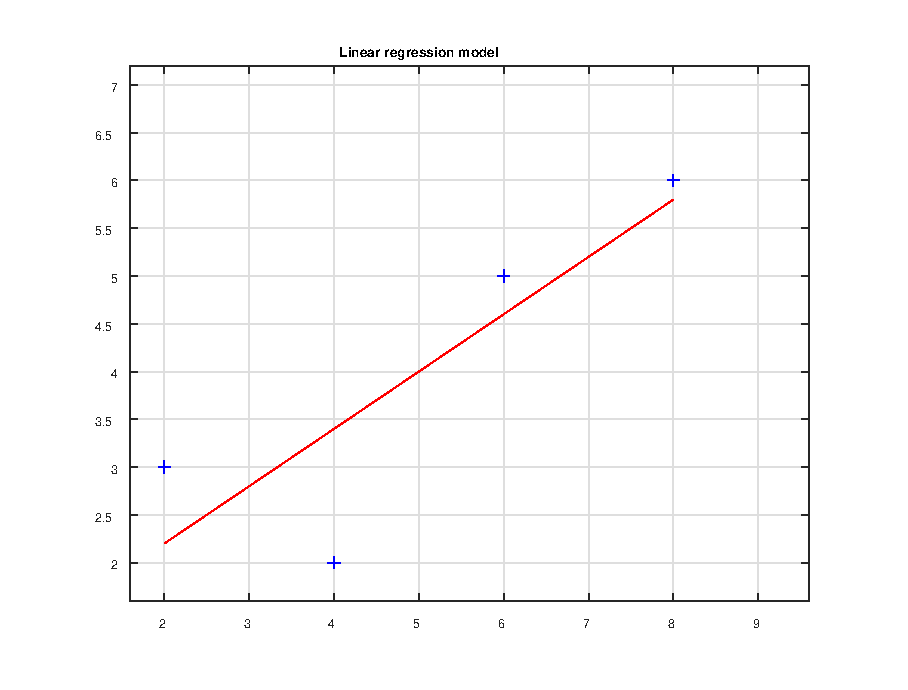
\includegraphics[width=\maxwidth{56.196688409433015em}]{figure_1.eps}
\end{center}

\label{H_9155F096}
\matlabheadingthree{Matrix resolution}

\begin{par}
\hfill \break
\end{par}

\begin{matlabcode}
beta = inv(X'*X)*X'*y
\end{matlabcode}
\begin{matlaboutput}
beta = 2x1    
    1.0000
    0.6000

\end{matlaboutput}
\begin{matlabcode}
y_est = beta(1) + beta(2)*x
\end{matlabcode}
\begin{matlaboutput}
y_est = 4x1    
    2.2000
    3.4000
    4.6000
    5.8000

\end{matlaboutput}
\begin{matlabcode}
plot(x,y,'b+',x,y_est,'r-')
xlim([min(x)*0.8,max(x)*1.2])
ylim([min(y)*0.8,max(y)*1.2])
title('Linear regression model')
grid on
\end{matlabcode}
\begin{center}
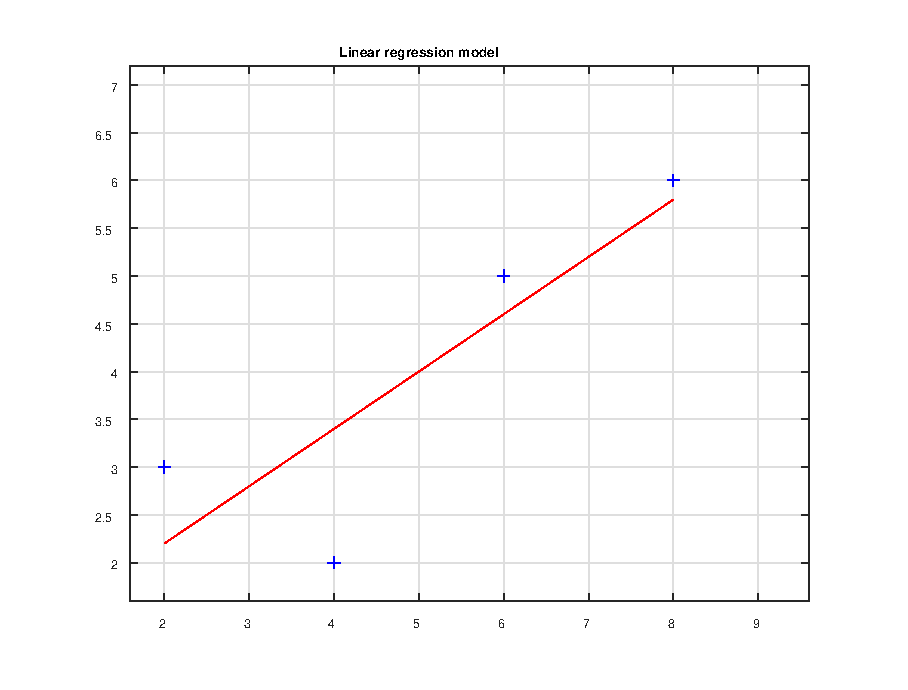
\includegraphics[width=\maxwidth{56.196688409433015em}]{figure_2.eps}
\end{center}

\begin{par}
\begin{flushleft}
As we can observe, the graph remains the same. Therefore, we can conclude that the problem is correctly solved.
\end{flushleft}
\end{par}


\label{H_9A3B1052}
\matlabheading{Exercise 2}

\begin{par}
\begin{flushleft}
Given the function
\end{flushleft}
\end{par}

\begin{par}
$$f\left(x\right)=x^3 -8x^2 +21x-18$$
\end{par}

\begin{par}
\begin{flushleft}
and knowing that it has a relative minimum in the interval \texttt{[2.8, 3.4]}, it is asked:
\end{flushleft}
\end{par}

\begin{par}
\begin{flushleft}
a) If you want to limit the solution to an interval of magnitude 0.01, what is the number of iterations necessary with the golden section algorithm? Design an algorithm to solve the problem.
\end{flushleft}
\end{par}

\begin{par}
\begin{flushleft}
b) With the same amplitude 0.01 of the final interval, what would be the number of iterations necessary with the Fibonacci algorithm? Design an algorithm to solve the problem.
\end{flushleft}
\end{par}

\begin{par}
\begin{flushleft}
c) Repeat this process with the bisection algorithm.
\end{flushleft}
\end{par}

\begin{par}
\begin{flushleft}
d) Solve this problem with MATLAB, use the \texttt{fminbnd} function as a method of search and the \texttt{fminunc} function as an iterative method.
\end{flushleft}
\end{par}

\label{H_46B8A91C}
\matlabheadingtwo{Solution}

\begin{par}
\begin{flushleft}
Plotting the function:
\end{flushleft}
\end{par}

\begin{matlabcode}
x = 2.8:0.01:3.4;
f = @(x) x.^3-8*x.^2+21.*x-18;

clf
figure(1)
plot(x,f(x))
xlim([2.8 3.4])
grid on
hold on
plot(3,0,'*r')
title('Representation of the function in the given interval')
\end{matlabcode}
\begin{center}
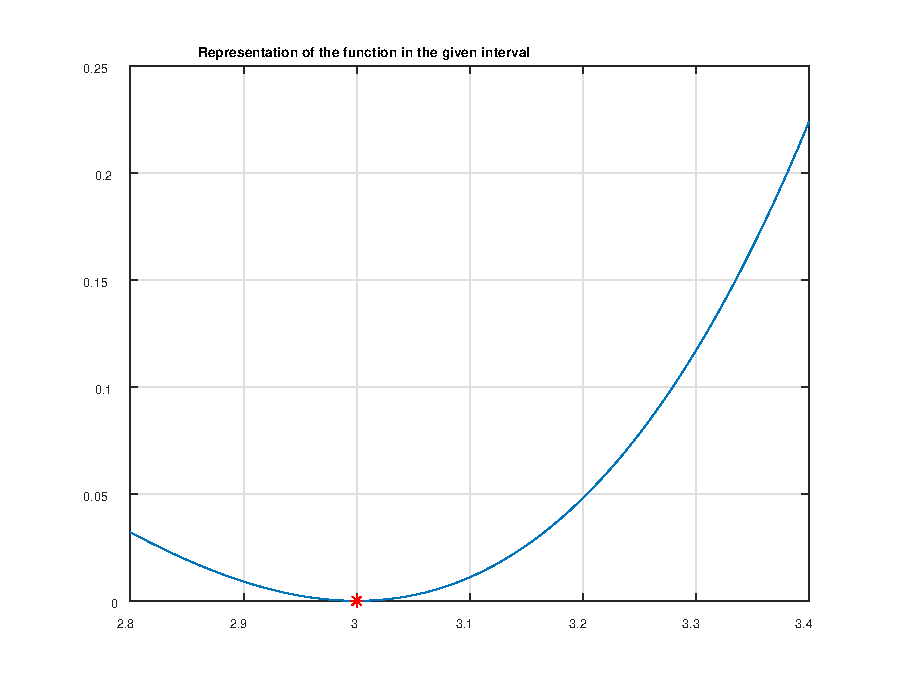
\includegraphics[width=\maxwidth{56.196688409433015em}]{figure_3.eps}
\end{center}

\begin{par}
\begin{flushleft}
a)  As we have seen in the notes, the number $n$ of iterations required to bound the length of the solution interval to $I_n <\epsilon$ is $n=\left\lceil \frac{\ln \left(I_0 \right)-\ln \left(\varepsilon \right)}{\ln \left(\phi \right)}\right\rceil$. Applied to our data:
\end{flushleft}
\end{par}

\begin{matlabcode}
ceil((log(3.4-2.8)-log(0.01))/log((1+sqrt(5))/2))
\end{matlabcode}
\begin{matlaboutput}
ans = 9
\end{matlaboutput}

\begin{par}
\begin{flushleft}
We will need \textbf{9 iterations}.
\end{flushleft}
\end{par}

\begin{par}
\begin{flushleft}
The new function is called \texttt{golden\_section(f,a,b,e)} and it takes the following parameters:
\end{flushleft}
\end{par}

\begin{itemize}
\setlength{\itemsep}{-1ex}
   \item{\begin{flushleft} \texttt{f} is the function that we want to find its optimal. \end{flushleft}}
   \item{\begin{flushleft} \texttt{a} is the lower bound of the search interval. \end{flushleft}}
   \item{\begin{flushleft} \texttt{b} is the upper bound of the search interval. \end{flushleft}}
   \item{\begin{flushleft} \texttt{e} is the admissible error limit (i.e.,\textit{ epsilon}, or the solution bound). \end{flushleft}}
\end{itemize}

\begin{matlabcode}
f = @(x) x.^3-8*x.^2+21.*x-18;
a = 2.8;
b = 3.4;
e = 0.01;

[a,b,k,sol] = golden_section(f,a,b,e)
\end{matlabcode}
\begin{matlaboutput}
a = 2.9957
b = 3.0036
k = 9
sol = 1x9    
    3.1708    2.9416    3.0833    3.0292    2.9751    3.0085    2.9878    2.9957    3.0036

\end{matlaboutput}
\begin{matlabcode}
clf
plot(x,f(x),'b-')
xlim([2.8 3.4])
title('Golden section search method')
grid on
hold on
plot(3,0,'*r')
hold on
plot(sol,f(sol),'ko')
\end{matlabcode}
\begin{center}
\includegraphics[width=\maxwidth{56.196688409433015em}]{figure_4.eps}
\end{center}

\begin{par}
\begin{flushleft}
\textbf{We can see that the algorithm needs 9 iterations} to stop until it has achieved a relatively good solution bound\textbf{. The interval is }\texttt{\textbf{[2.9957, 3.0036].}}
\end{flushleft}
\end{par}


\begin{par}
\begin{flushleft}
b) The new function is called fibonacci\_method\texttt{(f,a,b,e)}
\end{flushleft}
\end{par}

\begin{itemize}
\setlength{\itemsep}{-1ex}
   \item{\begin{flushleft} \texttt{f} is the function which we want to find its optimal. \end{flushleft}}
   \item{\begin{flushleft} \texttt{a} is the lower bound of the search interval. \end{flushleft}}
   \item{\begin{flushleft} \texttt{b} is the upper bound of the search interval. \end{flushleft}}
   \item{\begin{flushleft} \texttt{e} is the admissible error limit (i.e., \textit{epsilon}, or the solution bound). \end{flushleft}}
\end{itemize}

\begin{par}
\begin{flushleft}
To obtain the number of the Fibonacci terms needed (i.e., the number of iterations) it can be proved that the N+1-th term of the Fibonacci term should be greater than the size of the interval ($b-a$) and divided by the search interval size ($e$). In formal terms: $F_{N+1} \ge \left(b-a\right)\cdot \frac{1-2\epsilon }{e}$.
\end{flushleft}
\end{par}

\begin{par}
\begin{flushleft}
If we compute this expression we obtain:
\end{flushleft}
\end{par}

\begin{matlabcode}
n = (3.4-2.8)/0.01;     % criteria to obtain the last fibonacci term   
F = [1,2];              % initial values of fibonacci series

while F(end) < n
    F = [F,F(end)+F(end-1)];
end
\end{matlabcode}

\begin{par}
\begin{flushleft}
Seeing that we need 10 Fibonacci terms. Thus, \textbf{9 iterations are needed} (we must take into account that we compute up to the $N+1-\textrm{th}$ term, not up to the $N-\textrm{th}$ term). 
\end{flushleft}
\end{par}

\begin{par}
\begin{flushleft}
Indeed:
\end{flushleft}
\end{par}

\begin{matlabcode}
a = 2.8;
b = 3.4;
e = 0.01;

[a,b,k,sol] = fibonacci_method(f,a,b,e)
\end{matlabcode}
\begin{matlaboutput}
a = 2.9955
b = 3.0022
k = 9
sol = 1x9    
    3.1708    2.9416    3.0831    3.0292    2.9753    3.0090    2.9888    2.9955    3.0022

\end{matlaboutput}
\begin{matlabcode}
clf
plot(x,f(x),'b-')
xlim([2.8 3.4])
title('Fibonacci search method')
grid on
hold on
plot(3,0,'*r')
hold on
plot(sol,f(sol),'ko')
\end{matlabcode}
\begin{center}
\includegraphics[width=\maxwidth{56.196688409433015em}]{figure_5.eps}
\end{center}

\begin{par}
\begin{flushleft}
\textbf{We can affirm that the algorithm needs 9 iterations to stop until it has reached to a solution. The interval is [2.9955, 3.0022]}, slightly smaller to the previous interval. Since the number of iterations is very similar but the computational cost is higher, it does not worth to work with this algorithm for a problem with these features.
\end{flushleft}
\end{par}


\begin{par}
\begin{flushleft}
c)  As we have seen in the notes, the number of iterations will be the smallest integer $n$ satisfying:
\end{flushleft}
\end{par}

\begin{matlabcode}
ceil(-log(0.01/(3.4-2.8))/log(2))
\end{matlabcode}
\begin{matlaboutput}
ans = 6
\end{matlaboutput}

\begin{par}
\begin{flushleft}
The new function is called bisection\_method\texttt{(f,a,b,e)}
\end{flushleft}
\end{par}

\begin{itemize}
\setlength{\itemsep}{-1ex}
   \item{\begin{flushleft} \texttt{f} is the function which we want to find its optimal. \end{flushleft}}
   \item{\begin{flushleft} \texttt{a} is the lower bound of the search interval. \end{flushleft}}
   \item{\begin{flushleft} \texttt{b} is the upper bound of the search interval. \end{flushleft}}
   \item{\begin{flushleft} \texttt{e} is the admissible error limit (i.e., epsilon, or the solution bound). \end{flushleft}}
\end{itemize}

\begin{matlabcode}
clf
a = 2.8;
b = 3.4;
e = 0.01;

[a,b,k,sol] =bisection_method(f,a,b,e)
\end{matlabcode}
\begin{matlaboutput}
a = 2.9969
b = 3.0062
k = 6
sol = 1x6    
    3.1000    2.9500    3.0250    2.9875    3.0062    2.9969

\end{matlaboutput}
\begin{matlabcode}
plot(x,f(x),'b-')
xlim([2.8 3.4])
title('Bisection search method')
grid on
hold on
plot(3,0,'*r')
hold on
plot(sol,f(sol),'ko')
\end{matlabcode}
\begin{center}
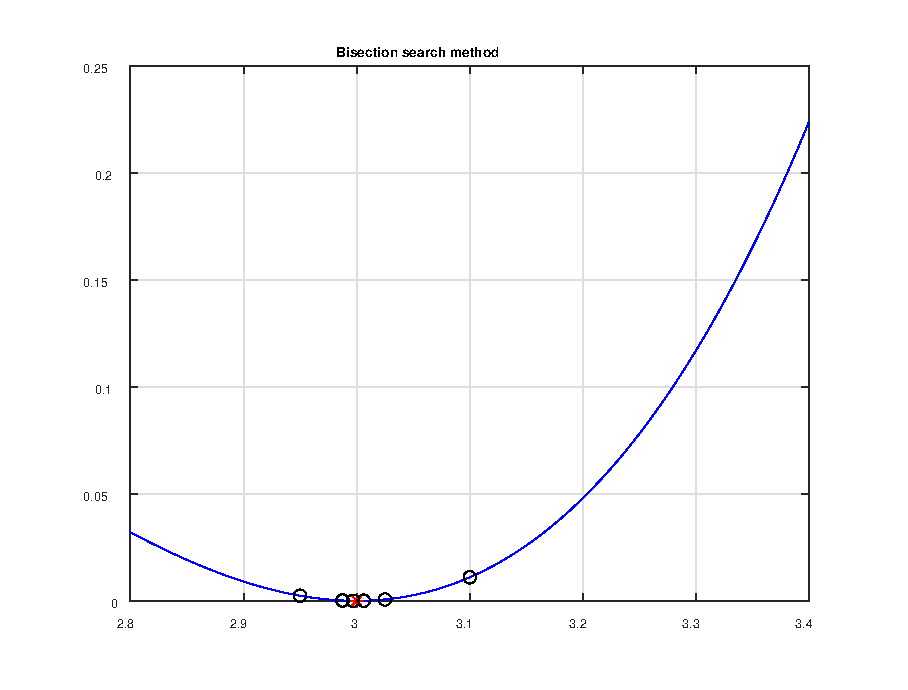
\includegraphics[width=\maxwidth{56.196688409433015em}]{figure_6.eps}
\end{center}

\begin{par}
\begin{flushleft}
As we can see, this search method is more efficient since it only \textbf{requires 6 iterations to reach the optimum}, which implies three fewer iterations than the two previous methods. We must take into account that despite this method converging more quickly, it requires computing the derivative, which is not always possible. Finally, the solution interval obtained is \textbf{[2.9969, 3.0062]}.
\end{flushleft}
\end{par}


\begin{par}
\begin{flushleft}
d) 
\end{flushleft}
\end{par}

\begin{matlabcode}
[x,fval,exit_flag,output] = fminbnd(f,2.8,3.4)
\end{matlabcode}
\begin{matlaboutput}
x = 3.0000
fval = 1.7550e-12
exit_flag = 1
output = 
    iterations: 7
     funcCount: 8
     algorithm: 'golden section search, parabolic interpolation'
       message: 'Optimization terminated:↵ the current x satisfies the termination criteria using OPTIONS.TolX of 1.000000e-04 ↵'

\end{matlaboutput}
\begin{matlabcode}
[x,fval,exit_flag,output] = fminunc(f,2.8)
\end{matlabcode}
\begin{matlaboutput}
Local minimum found.

Optimization completed because the size of the gradient is less than
the value of the optimality tolerance.

<stopping criteria details>
x = 3.0000
fval = 7.1054e-15
exit_flag = 1
output = 
       iterations: 6
        funcCount: 14
         stepsize: 7.9427e-07
     lssteplength: 1
    firstorderopt: 0
        algorithm: 'quasi-newton'
          message: 'Local minimum found.↵↵Optimization completed because the size of the gradient is less than↵the value of the optimality tolerance.↵↵<stopping criteria details>↵↵Optimization completed: The first-order optimality measure, 0.000000e+00, is less ↵than options.OptimalityTolerance = 1.000000e-06.'

\end{matlaboutput}

\begin{par}
\begin{flushleft}
The pre-built functions give the exact optimal value. But as we can see, \textbf{the }\texttt{\textbf{fminbnd}}\textbf{ method} (based on the golden section search algorithm with parabolic interpolation) \textbf{takes 7 iterations to converge}. Meanwhile, \textbf{the }\texttt{\textbf{fminunc}}\textbf{ method} (based on a variant of a gradient descent method) \textbf{takes 6 iterations}.
\end{flushleft}
\end{par}


\label{H_8BA87314}
\matlabheading{Exercise 3}

\begin{par}
\begin{flushleft}
Given the function
\end{flushleft}
\end{par}

\begin{par}
$$f\left(x_1 ,x_2 \right)=x_1^2 +3x_2^2 +\left(x_1 -2\right)\left(x_2 -3\right)$$
\end{par}

\begin{par}
\begin{flushleft}
Starting from the origin of coordinates, the following is requested:
\end{flushleft}
\end{par}

\begin{par}
\begin{flushleft}
a) Determine the direction of steepest descent. 
\end{flushleft}
\end{par}

\begin{par}
\begin{flushleft}
b) Perform a couple of iterations with the Steepest Descent algorithm. 
\end{flushleft}
\end{par}

\begin{par}
\begin{flushleft}
c) Perform a couple of iterations with the Newton algorithm. 
\end{flushleft}
\end{par}

\begin{par}
\begin{flushleft}
d) Solve the unconstrained minimization problem using Matlab; you can use the fminsearch function.
\end{flushleft}
\end{par}

\label{H_2E30E861}
\matlabheadingtwo{Solution}

\label{H_E90DE5EE}
\matlabheadingthree{Representation of the function}

\begin{par}
\hfill \break
\end{par}

\begin{matlabcode}
feval = @(x,y) x.^2 + 3*y.^2 + (x - 2).*(y - 3);
[Xgrid,Ygrid]=meshgrid(-3:0.1:3,-3:0.1:3);
z = feval(Xgrid,Ygrid);

figure(1)
clf
surface(Xgrid,Ygrid,z)
view(45,45)
title('f(x_1,x_2)')
xlabel('x_1')
ylabel('x_2')
\end{matlabcode}
\begin{center}
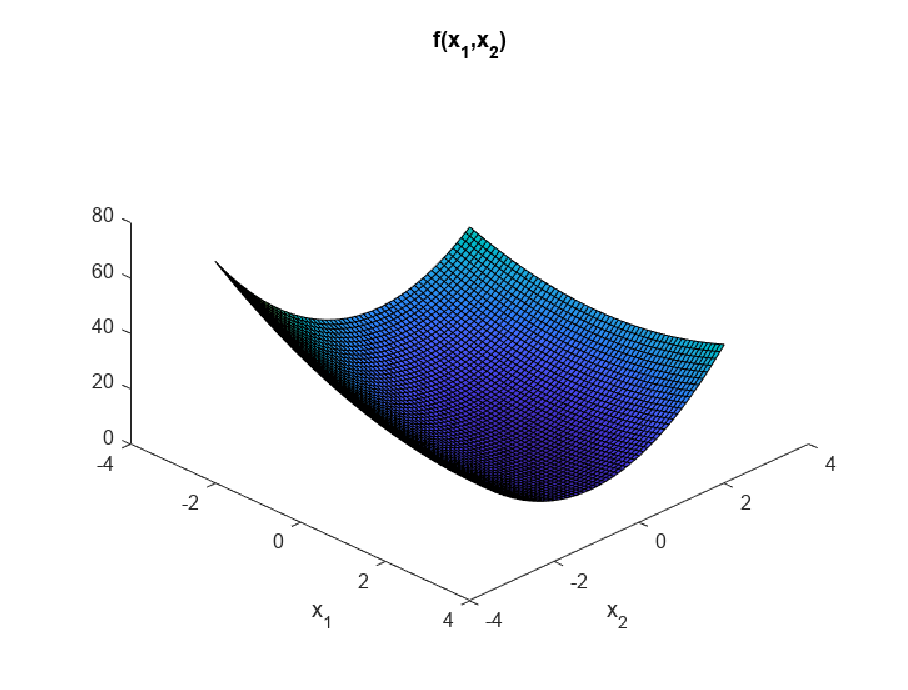
\includegraphics[width=\maxwidth{56.196688409433015em}]{figure_7.eps}
\end{center}


\begin{par}
\begin{flushleft}
a) The direction of the steepest descent in an arbitrary point $\left(x_1 ,x_2 \right)\;$ is $\nabla f\left(x_1 ,x_2 \right)=\left\lbrack \begin{array}{l}
2x_1 +\left(x_2 -3\right)\\
6x_2 +\left(x_1 -2\right)
\end{array}\right\rbrack$, $\nabla f\left(0,0\right)=-\left\lbrack \begin{array}{l}
3\\
2
\end{array}\right\rbrack$. Normalizing:
\end{flushleft}
\end{par}

\begin{matlabcode}
clc
syms x y;
f = x.^2 + 3*y.^2 + (x - 2).*(y - 3)
\end{matlabcode}
\begin{matlabsymbolicoutput}
f = 

\hskip1em $\displaystyle {\left(x-2\right)}\,{\left(y-3\right)}+x^2 +3\,y^2 $
\end{matlabsymbolicoutput}
\begin{matlabcode}
grad=gradient(f,[x,y]);

V = subs(grad, [x, y], [0, 0]);
d = -(V/norm(V));
round(d,4)
\end{matlabcode}
\begin{matlabsymbolicoutput}
ans = 

\hskip1em $\displaystyle \left(\begin{array}{c}
0.8321\\
0.5547
\end{array}\right)$
\end{matlabsymbolicoutput}

\begin{par}
\begin{flushleft}
b) 
\end{flushleft}
\end{par}

\begin{matlabcode}
clc
syms x y;
f = x.^2 + 3*y.^2 + (x - 2).*(y - 3);
grad = gradient(f,[x, y]);

n=2;
sol = zeros(n+1,2);
for i=2:n+1
    V = subs(grad, [x, y], [sol(i-1,1),sol(i-1,2)]);
    d = -(V/norm(V));
    syms l;
    g = simplify(subs(f, [x, y], [sol(i-1,1)+l*d(1),sol(i-1,2)+l*d(2)]));
    gd = diff(g);
    l = round(solve(gd),4);
    sol(i,:) = sol(i-1,:)'+round(l*d,4);
end

display(sol)
\end{matlabcode}
\begin{matlaboutput}
sol = 3x2    
         0         0
    0.7222    0.4815
    1.0015    0.0626

\end{matlaboutput}

\begin{par}
\begin{flushleft}
As we can see, we obtain in the first iteration the approximations $\left\lbrack x_1 ,x_2 \right\rbrack =\left\lbrack 0\ldotp 7222,0\ldotp 4815\right\rbrack$, meanwhile in the second iteration we have obtained $\left\lbrack x_1 ,x_2 \right\rbrack =\left\lbrack 1\ldotp 0015,0\ldotp 0626\right\rbrack$. If we represent both solutions:
\end{flushleft}
\end{par}

\begin{matlabcode}
figure(1)
hold on
title('Steepest Descent algorithm')
b = plot3(sol(:,1),sol(:,2),feval(sol(:,1),sol(:,2)),'r*');
\end{matlabcode}
\begin{center}
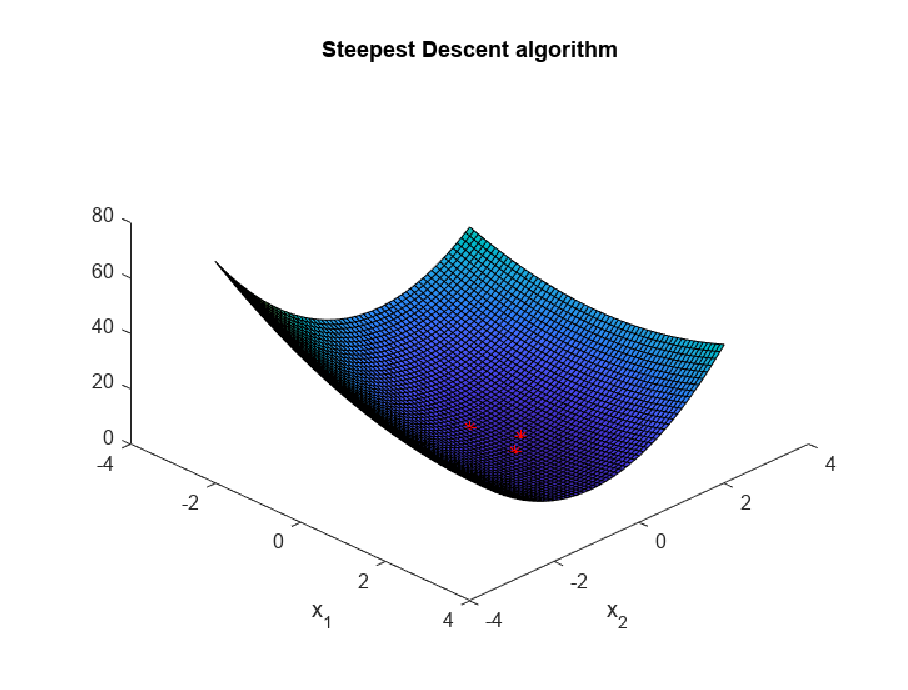
\includegraphics[width=\maxwidth{56.196688409433015em}]{figure_8.eps}
\end{center}


\begin{par}
\begin{flushleft}
c) 
\end{flushleft}
\end{par}

\begin{matlabcode}
clc
syms x y;
f = x.^2 + 3*y.^2 + (x - 2)*(y - 3);
grad = gradient(f,[x,y]);
hess = hessian(f,[x,y]);

n=2;
sol = zeros(n+1,2);
for i=2:n+1
    V = subs(grad, [x, y], [sol(i-1,1),sol(i-1,2)]);
    H = subs(hess, [x, y], [sol(i-1,1),sol(i-1,2)]);
    sol(i,:) = sol(i-1,:)'-inv(H)*V;
end

display(sol)
\end{matlabcode}
\begin{matlaboutput}
sol = 3x2    
         0         0
    1.4545    0.0909
    1.4545    0.0909

\end{matlaboutput}
\begin{matlabcode}
figure(1)
hold on
delete(b)
title('Newton algorithm')
c = plot3(sol(:,1),sol(:,2),feval(sol(:,1),sol(:,2)),'r*');
\end{matlabcode}
\begin{center}
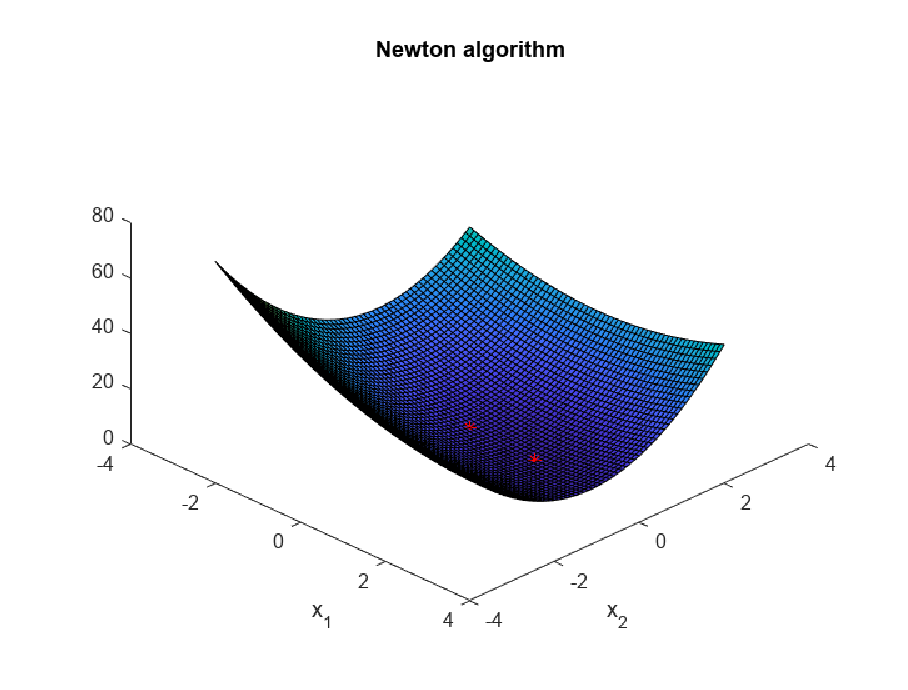
\includegraphics[width=\maxwidth{56.196688409433015em}]{figure_9.eps}
\end{center}

\begin{par}
\begin{flushleft}
We always will reach the minimum in \textbf{one iteration} because $f\left(x_1 ,x_2 \right)$ is a quadratic function. 
\end{flushleft}
\end{par}

\begin{par}
\begin{flushleft}
d) 
\end{flushleft}
\end{par}

\begin{matlabcode}
f3 =@(x) x(1)^2 + 3*x(2)^2 + (x(1) - 2)*(x(2) - 3);
[x,fval,exit_flag,output]=fminsearch(f3,[0;0])
\end{matlabcode}
\begin{matlaboutput}
x = 2x1    
    1.4545
    0.0909

fval = 3.7273
exit_flag = 1
output = 
    iterations: 58
     funcCount: 110
     algorithm: 'Nelder-Mead simplex direct search'
       message: 'Optimization terminated:↵ the current x satisfies the termination criteria using OPTIONS.TolX of 1.000000e-04 ↵ and F(X) satisfies the convergence criteria using OPTIONS.TolFun of 1.000000e-04 ↵'

\end{matlaboutput}

\begin{par}
\begin{flushleft}
This method takes \textbf{58 iterations} until termination (which is a much higher number of iterations compared with the other algorithms).
\end{flushleft}
\end{par}

\end{document}
